%! Author = itgramic
%! Date = 05.12.23

% Preamble
\begin{flushleft}
    \subsubsection{CloudNativePG}
    CloudNativePG ist eine Containerlösung für PostgreSQL auf Kubernetes.\\
    CloudNativePG wurde ursprünglich von EDB entwickelt.
\end{flushleft}
\begin{flushleft}
    \paragraph{Core-Features}
    Die wichtigsten Features von CloudNativePG sind\cite{5ALQPE2U}:
    \begin{itemize}
        \item k8s API integration
        \item Autoamtischer Failover
        \item Self-Healing von Nodes resp. Replikas
        \item Skalierbarkeit (Vertikal, Horizontal bedingt)
        \item Volumne Backup
        \item Object Backup
        \item Rolling PostgreSQL Upgrade / Updates
        \item Pooling mit PgBouncer
        \item Offline und Online Import von bestehenden PostgreSQL DBs
    \end{itemize}
\end{flushleft}
\begin{flushleft}
    \paragraph{Replikation}
    CloudNativePG bietet die üblichen PostgreSQL Replikaionen an.
\end{flushleft}
\begin{flushleft}
    \paragraph{Proxy}
    CloudNativePG benötigt keinen zusätzlichen Proxy.
\end{flushleft}
\begin{flushleft}
    \paragraph{Pooling}
    CloudNativePG unterstützt pgBouncer als Pooler.
\end{flushleft}
\begin{flushleft}
    \paragraph{API / Skripte}
    CloudNativePG bietet eine API zum Monitoren und Verwalten von Backups, Clustern und dem System selbst\cite{LY8V4XQM}.
\end{flushleft}
\begin{flushleft}
    \paragraph{Architektur}
    Kubernetes regelt die Zugriffe mittels eines entsprechenden Services in die Nodes auf den Pods:
    \begin{figure}[H]
        \centering
        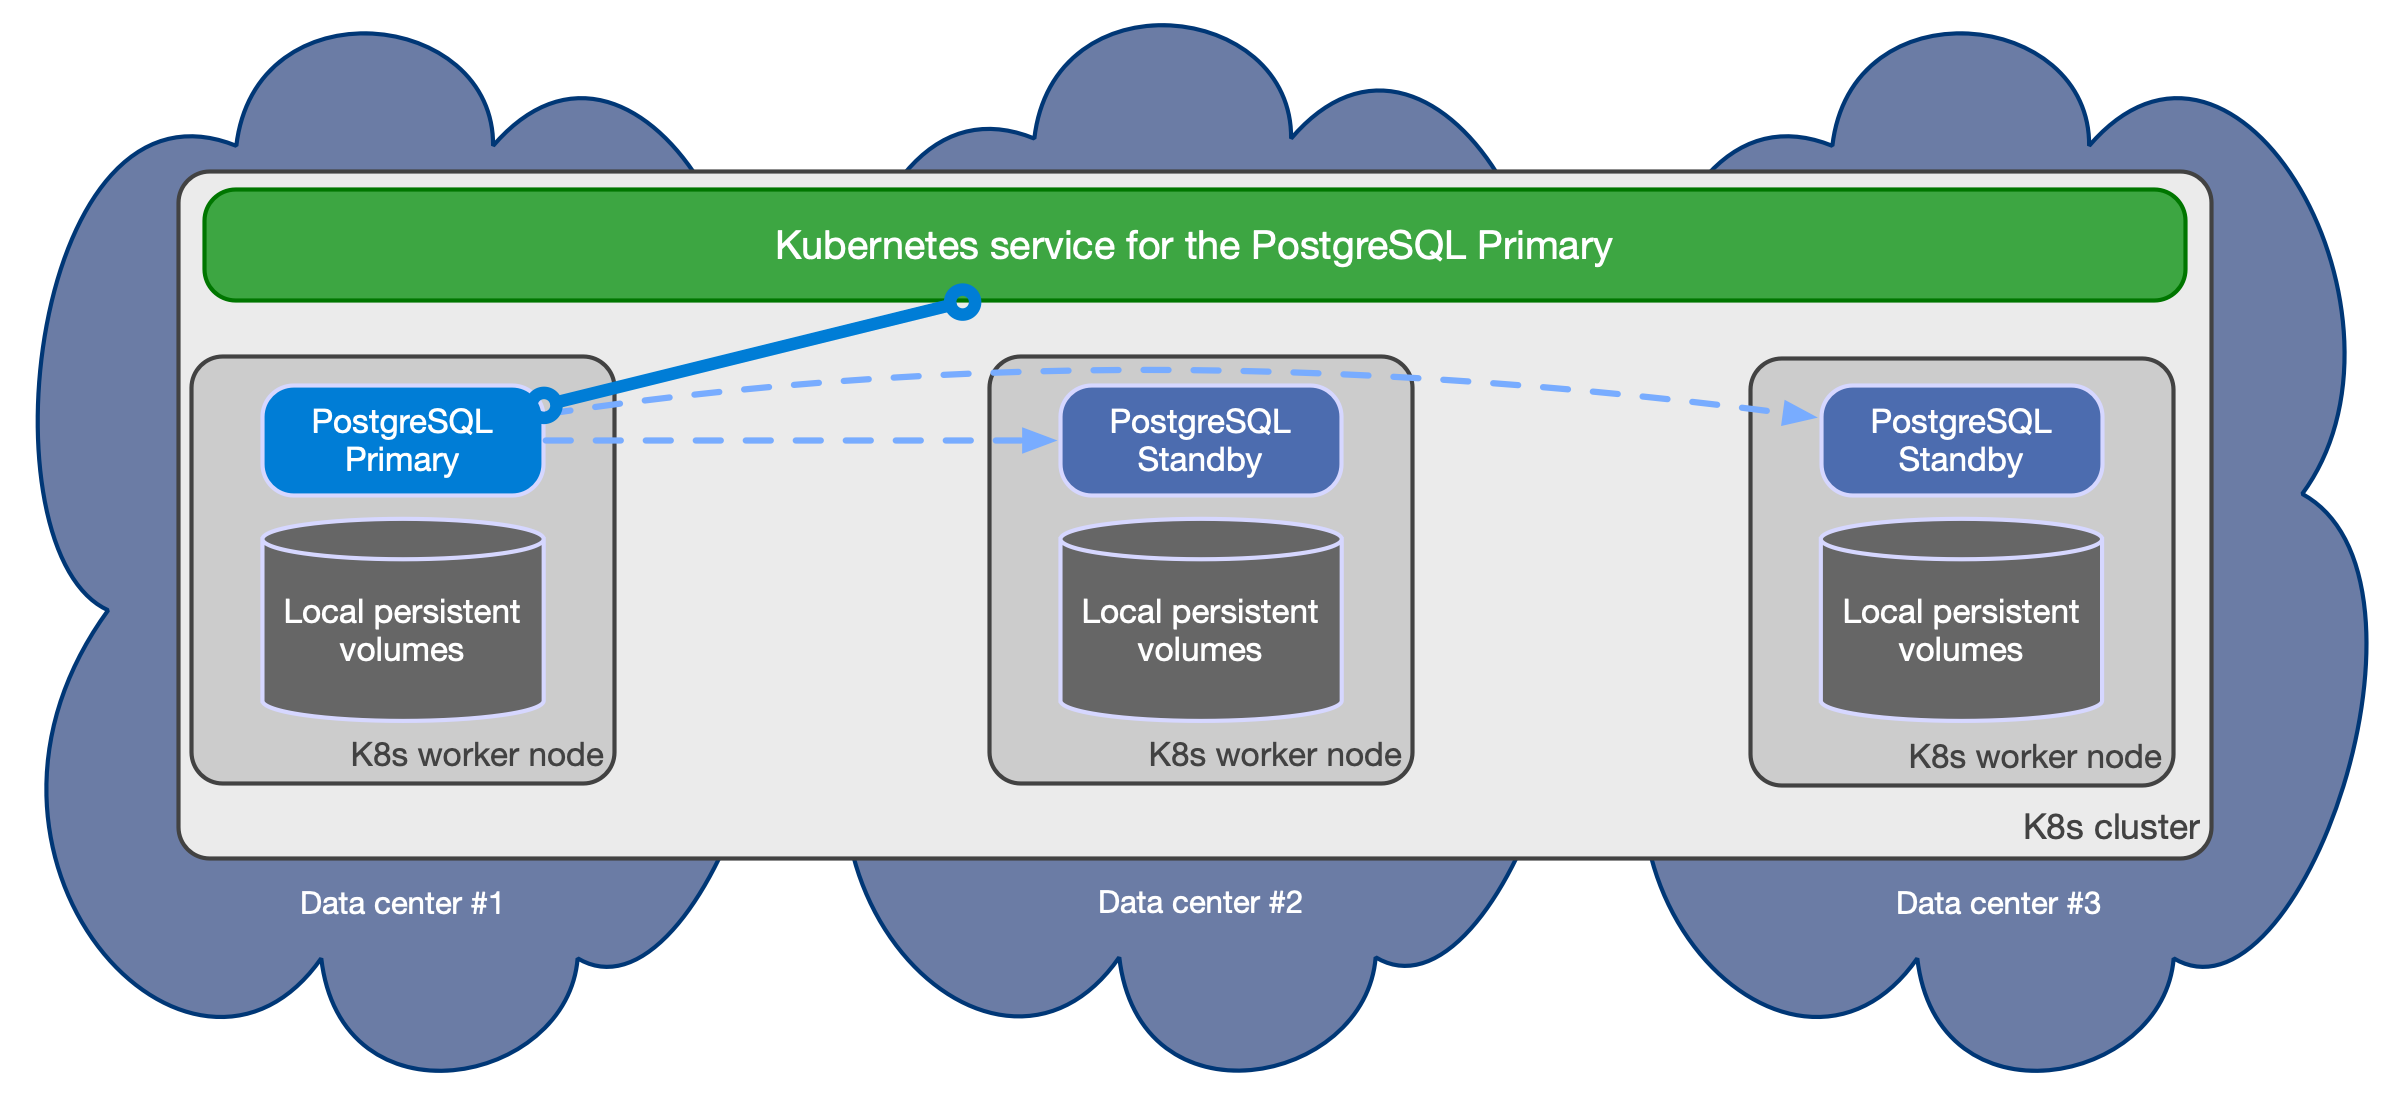
\includegraphics[width=0.75\linewidth]{source/implementation/evaluation/postgresql_ha_solutions/cloudnativepg/k8s-pg-architecture}
        \caption{CloudNativePG - Kubernetes - PostgreSQL}
        \label{fig:k8s-pg-architecture}
    \end{figure}
\end{flushleft}
\begin{flushleft}
    Dabei werden die Read-write workloads an den Primary Node gesendet:
    \begin{figure}[H]
        \centering
        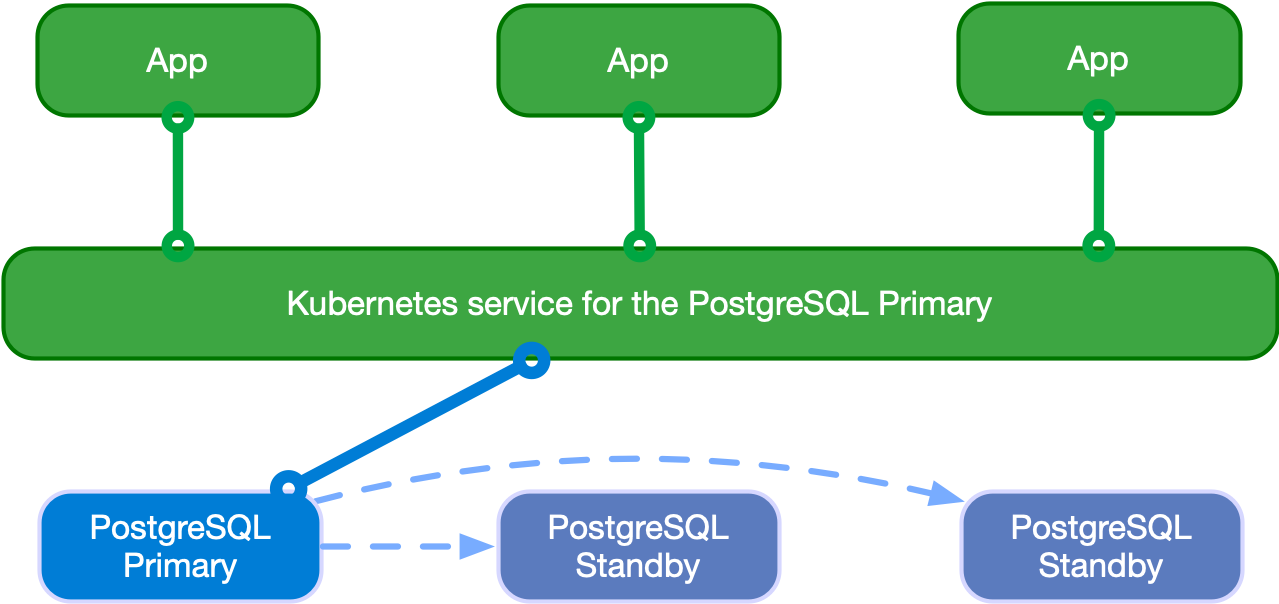
\includegraphics[width=0.75\linewidth]{source/implementation/evaluation/postgresql_ha_solutions/cloudnativepg/cloudnativepg-architecture-rw}
        \caption{CloudNativePG - Kubernetes - Read-write workloads}
        \label{fig:cloudnativepg-architecture-rw}
    \end{figure}
\end{flushleft}
\begin{flushleft}
    Read-only workloads werden mit Round robin an die Replicas zugewiesen:
    \begin{figure}[H]
        \centering
        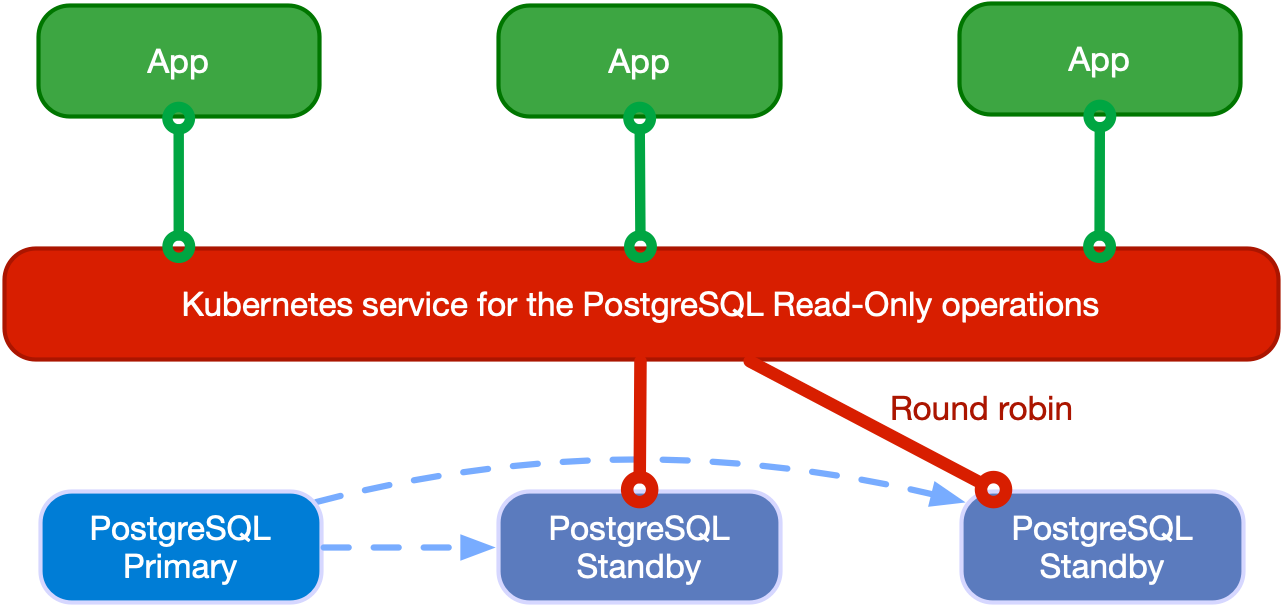
\includegraphics[width=0.75\linewidth]{source/implementation/evaluation/postgresql_ha_solutions/cloudnativepg/cloudnativepg-architecture-read-only}
        \caption{CloudNativePG - Kubernetes - Read-only workloads}
        \label{fig:cloudnativepg-architecture-read-only}
    \end{figure}
\end{flushleft}
\begin{flushleft}
    Es könnten auch Lösungen mit Designated Kubernetes-Clustern in einem anderen RZ oder einer anderen Geo-Region realisiert werden.
\end{flushleft}
\begin{flushleft}
    \paragraph{Maintenance}
    Das Projekt hat eine relativ hohe Anzahl an aktiven Issues, wobei viele neue dazugekommen sinned:
    \begin{figure}[H]
        \centering
        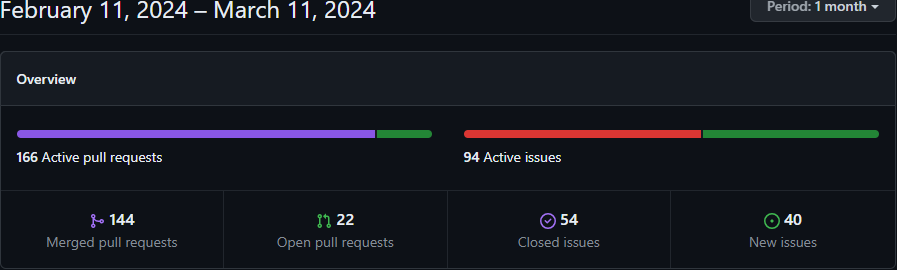
\includegraphics[width=0.75\linewidth]{source/implementation/evaluation/postgresql_ha_solutions/insights/cloudnativepg/pulse_cloudnative-pg_cloudnative-pg}
        \caption{CloudNativePG - Pulse}
        \label{fig:pulse_cloudnative-pg_cloudnative-pg}
    \end{figure}

    Der Code ist aber recht gut gepflegt, Code wird nicht nur regelmässig hinzugefügt, sondern auch entfernt.
    Auffällig ist, das im April 2022 eine grosse Menge Code entfernt wurde:
    \begin{figure}[H]
        \centering
        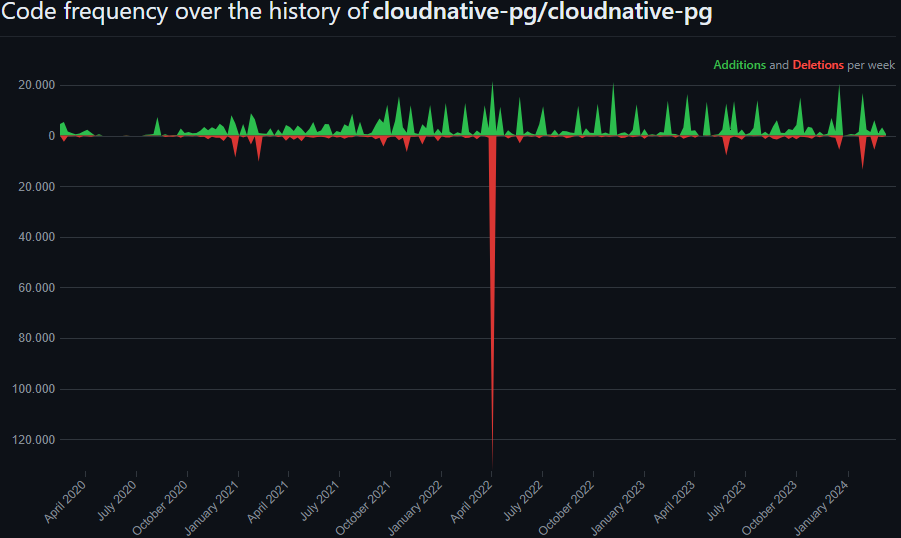
\includegraphics[width=0.75\linewidth]{source/implementation/evaluation/postgresql_ha_solutions/insights/cloudnativepg/code_frequency_cloudnative-pg_cloudnative-pg}
        \caption{CloudNativePG - Code Frequency}
        \label{fig:code_frequency_cloudnative-pg_cloudnative-pg}
    \end{figure}

    Das Projekt hält die meisten Standards von GitHub ein:
    \begin{figure}[H]
        \centering
        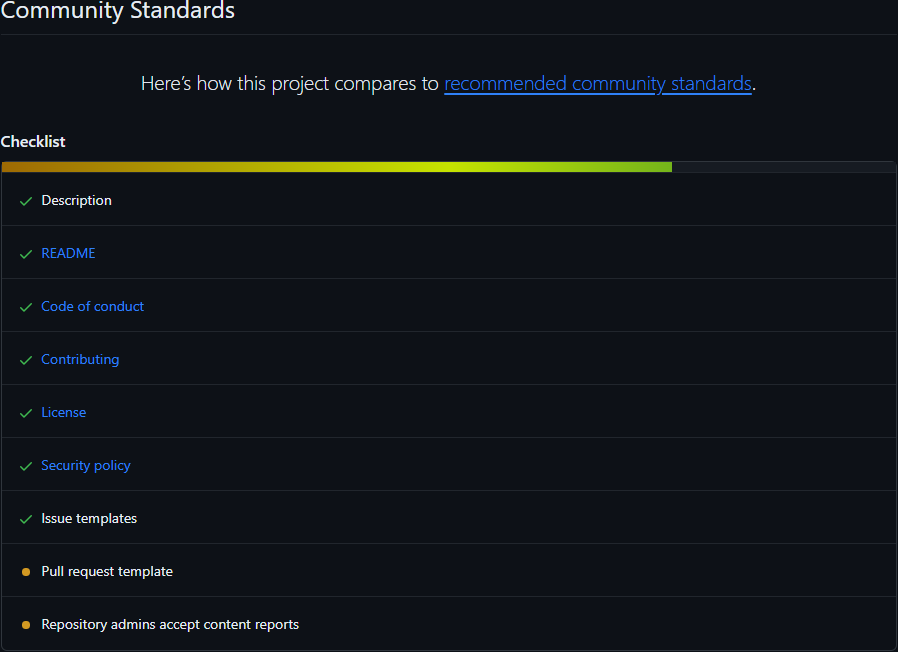
\includegraphics[width=0.75\linewidth]{source/implementation/evaluation/postgresql_ha_solutions/insights/cloudnativepg/community_standards}
        \caption{CloudNativePG - Community Standards}
        \label{fig:community_standards_cloudnativepg}
    \end{figure}

    Die Contributors committen zwar Regelmässig auf das Projekt, allerdings fügen sie ungleich mehr dazu als sie alten Code bereinigen.\\
    Das führt dann dazu, dass es dann zu grösseren Aufräumarbeiten kommt wie im April 2022.\\
    Es kann der Eindruck gewonnen werden, dass der Code wenig aufgeräumt wird und viel Balast mit sich schleppt,\\
    was ein Sicherheitsrisiko darstellen kann:
    \begin{figure}[H]
        \centering
        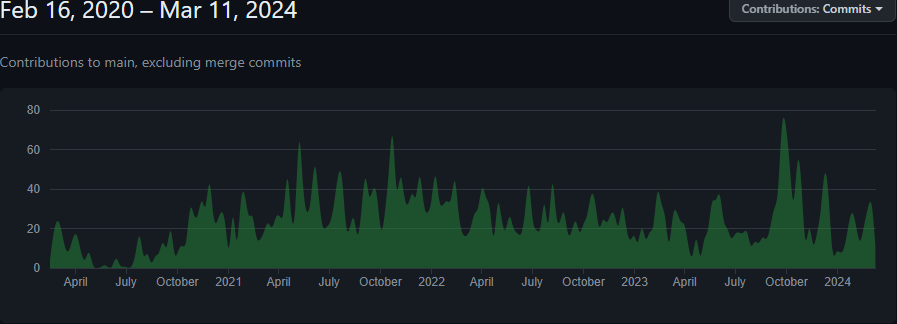
\includegraphics[width=0.75\linewidth]{source/implementation/evaluation/postgresql_ha_solutions/insights/cloudnativepg/contributors_commits_cloudnative-pg_cloudnative-pg}
        \caption{CloudNativePG - Contributors Commits}
        \label{fig:contributors_commits_cloudnative-pg_cloudnative-pg}
    \end{figure}
    \begin{figure}[H]
        \centering
        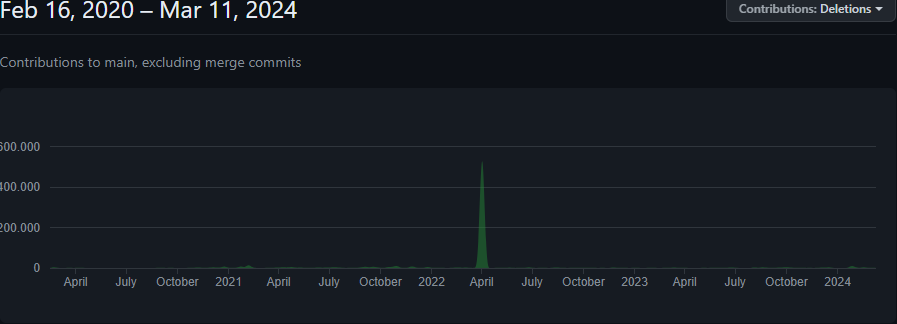
\includegraphics[width=0.75\linewidth]{source/implementation/evaluation/postgresql_ha_solutions/insights/cloudnativepg/contributors_deletations_cloudnative-pg_cloudnative-pg}
        \caption{CloudNativePG - Contributors Deletations}
        \label{fig:contributors_deletations_cloudnative-pg_cloudnative-pg}
    \end{figure}
    \begin{figure}[H]
        \centering
        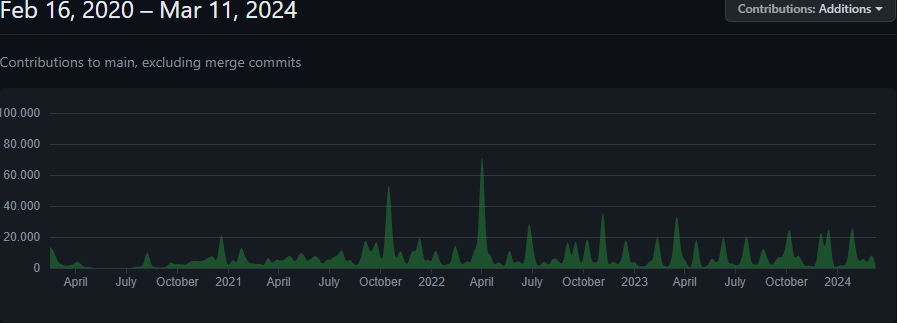
\includegraphics[width=0.75\linewidth]{source/implementation/evaluation/postgresql_ha_solutions/insights/cloudnativepg/contributors_additions_cloudnative-pg_cloudnative-pg}
        \caption{CloudNativePG - Contributors Additions}
        \label{fig:contributors_additions_cloudnative-pg_cloudnative-pg}
    \end{figure}

    Commits werden regelmässig abgesetzt, allerdings gibt es immer wieder gehäufte Commits.\\
    Oft um die Monatswechsel herum:
    \begin{figure}[H]
        \centering
        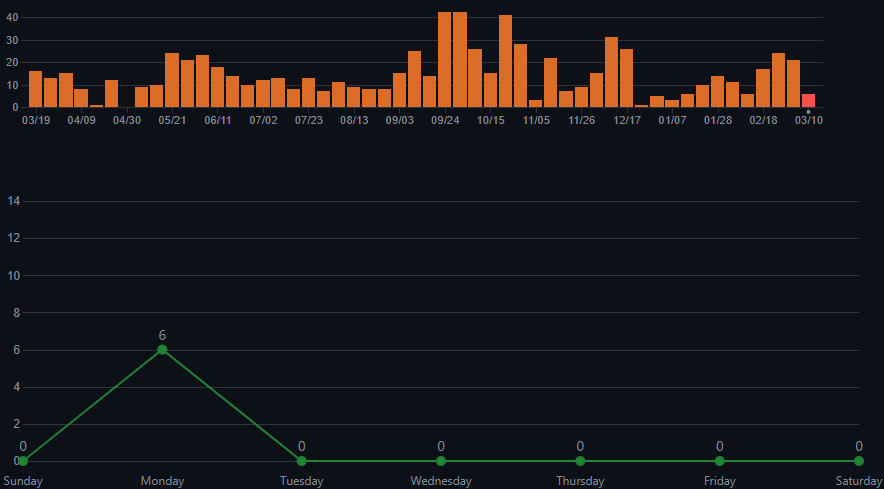
\includegraphics[width=0.75\linewidth]{source/implementation/evaluation/postgresql_ha_solutions/insights/cloudnativepg/commit_activity_cloudnative-pg_cloudnative-pg}
        \caption{CloudNativePG - Commit Activity}
        \label{fig:commit_activity_cloudnative-pg_cloudnative-pg}
    \end{figure}

    Nebst dem Projekt cloudnative-pg der \guillemotleft© The CloudNativePG Contributors\guillemotright ist CloudNativePG-Gründer EDB noch immer ein grosser Contributor.
     \begin{figure}[H]
        \centering
        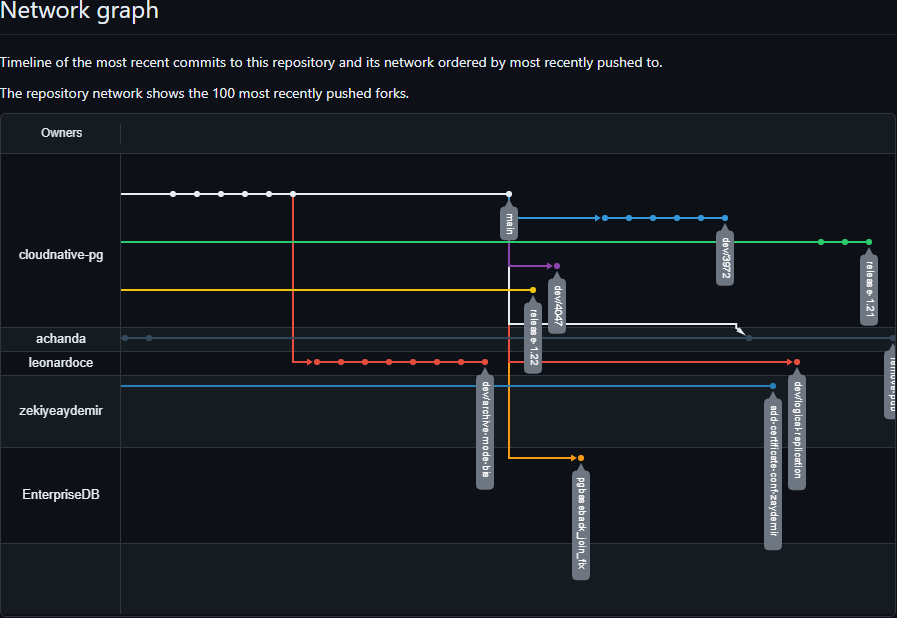
\includegraphics[width=0.75\linewidth]{source/implementation/evaluation/postgresql_ha_solutions/insights/cloudnativepg/network_graph_cloudnative-pg_cloudnative-pg}
        \caption{CloudNativePG - Network Graph}
        \label{fig:network_graph_cloudnative-pg_cloudnative-pg}
    \end{figure}
\end{flushleft}
\begin{flushleft}
    \paragraph{Synergien und Mehrwert}
    CloudNativePG bleibt ein Monolithisches System,\\welches aber keine Möglichkeit bietet,\\auch auf einem Normalen Serversetting betrieben zu werden.
\end{flushleft}
\begin{flushleft}
    Daher bietet CloudNativePG weder einen Benefit durch seine Architektur noch mit der Möglichkeit,\\Synergien nutzen zu können.
\end{flushleft}